\chapter{Experimentaci\'on y Resultados}\label{chapter:experiments}
% Expandir los outlines de esto
\section{Marco Experimental}

En este secci\'on se analiza el desemepe\~no de la propuesta utilizando AutoGOAL.

El objetivo es ejecutar datasets distintos con diferentes m\'etricas de evaluaci\'on.

\subsection{M\'etricas Utilizadas}

Para cada conjutno de datos se utilizan los siguentes pares de m\'etricas:

\paragraph{Precision contra Recobrado}: Precisi\'on es cuando . Recobrado es cuando . Para los tests donde se utiliza de una manera. Y para otros de otra

\paragraph{F-Score contra Tiempo de Entrenamiento}: Se compara F-Score lo mismo que Recobrado y Precision. Para algunos tests de alguna forma, para otros de otra. Tiempo de Entrenemaiento es un estimado de cuanto timepo toma entrenar y validar el modelo.

\subsection{Corpus de Evaluaci\'on}

Se utilizan dos corpus de datos para comprobar el comportamiento del sistema cuando optmiza para varias m\'etricas simult\'aneamente.

\subsubsection{CARS}
Cars representa una conjunto de carros y con ciertas caracter\'isticas cat\'alogadas cualitativamente (ver \ref{implementation:table:cars:attributes}). Cada carro se clasifica de acuerdo a sus atributos  en inaceptable, aceptable, bueno o muy bueno (\ref{implementation:table:cars:classes}). El dataset no tiene valores desconocidos.

\begin{table}[ht]
    \centering
    \parbox{.45\linewidth}{
    \begin{tabular} { |l|c| }
        \hline
        Atributos & Valores \\
        \hline
        \hline
        buying & v-high, hihg, med, low \\
        \hline
        maintance &  v-high, hihg, med, low\\
        \hline
        doors & 2, 3, 4, 5-more\\
        \hline
        persons & 2, 4, more\\
        \hline
        lug\_boot & small, med, big\\
        \hline
        safety & low, med, high\\
        \hline
    \end{tabular}
    \caption{Tipos de Atributos en Cars}
    \label{implementation:table:cars:attributes}
    }
    \qquad
    \parbox[t]{.45\linewidth}{
    \begin{tabular} {|l|c|c|}
        \hline
        Clases & N & \% \\
        \hline
        \hline
        unacc & 1210 & 70.023\%\\
        \hline
        acc & 384 & 22.222\%\\
        \hline
        good & 69 & 3.993\%\\
        \hline
        v-good & 65 & 3.762\%\\
        \hline
    \end{tabular}
    \caption{Distribuci\'on de clases en Cars}
    \label{implementation:table:cars:classes}
    }
\end{table}

\subsubsection{HAHA}
Humor Analysis based on Human Annotation (HAHA), un conjunto de datos que contiene \textit{tweets} en espa\~nol y se clasifican en si son humor\'isticos o no. Contiene un total de 30000 tweets donde se utilizan 24000 para entrenaiento y 6000 para evaluaci\'on.

\begin{table}[ht]
    \centering
    \begin{tabular} {|l||c|c|c|}
        \hline
        & Entrenamiento & Evaluaci\'on & Total \\
        \hline
        \hline
        Tweets & 24000 & 6000 & $30000$\\
        \hline
        Graciosos & 9253 & 2342 & 11595\\
        \hline
        No graciosos & 14 757 & 3 658 & 18 405\\
        \hline
        Puntuaci\'on Promedio & 1305 & 275 & 1580\\
        \hline
    \end{tabular}
    \caption{Distribuci\'on de clases en HAHA}
    \label{implementation:table:haha}
\end{table}

\subsubsection{MEDDOCAN}

Una colecci\'on de 1000 casos cl\'inicos y sus anotaciones PHI; cada uno conformado con aproximadamente de 33 oraciones o 495 palabras. Cada caso cl\'inico est\'a codificado en texto plano en UTF8 y las anotaciones est\'an en formato BRAT.


\subsection{Configuraci\'on Experimental}

\paragraph{Hardware} Los experimentos fueron ejecutados en un equipo con las siguientes propiedades: CPU AMD R5 3550h y 32 GB de RAM.

\section{Resultados y An\'alisis}

A continuaci\'on se muestran los resultados y anal\'isi de aplicar autogoal con optimizaci\'on multiobjetivo a los distintos corpus. En las gr\'aficas solo se tiene en cuenta la puntuaci\'on respecto a los datos entrenamiento y no a los datos de prueba. Los puntos con tonalidades de grises marcan las mejores soluciones encontradas en cada generaci\'on que realiz\'o el sistema. La tonalidad de los puntos oscurecen a medida que han sido m\'as generaciones. Las puntos m\'as oscuros corresponden a iteraciones posteriores. Finalmente los puntos marcados con cruces rojas representan las mejores soluciones encontradas por el algoritmo y conforman una aproximaci\'on del frente de Pareto.

\subsection{Cars}

Se utilzo una poblacion total de 40 individuos, 1 hora de tiempo m\'aximo y 10 segundos de tiempo l\'imite por \textit{pipeline}. Se utilizaron las la implementaciones de \textit{f-score}, \textit{precision} y \textit{recall} de scikit-learn con el promedio \textit{weighted} utilizado para problemas de clasificaci\'on multiclase que pueden tener un desbalance en las clases existentes.

\subsubsection{F-Score contra Tiempo de Entrenamiento}

En la figura \ref{impl:fig:cars:fscore_vs_time} se observa que se obtiene una porci\'on aproximaci\'on del frente de Pareto bien distribuida. Se nota lo que se conoce en la literatura como un frente c\'oncavo. Ademas se puede ver como se tienen solucioens para escoger/ Desde cercanas a los milisegundos con una puntuaci\'on de 0.9, o que se peguen a los 0.2 milisegundos con una puntacion f casi perfecta. En este caso la diferencia de tiempe es negligible. No obstante al optimziar sim\'ulataneamete para el tiempo se evita que el algoritmo escoja caminos m\'as caros en tiempo como se ve en la columna de puntos a la derecha. Varios algoritmos con muy buena puntuaci\'on pero que se demoran 5 veces m\'as que el m\'as r\'apido.

% (hablar sobre los mejores algorimtos)?

\begin{figure}[ht]
    \centering
    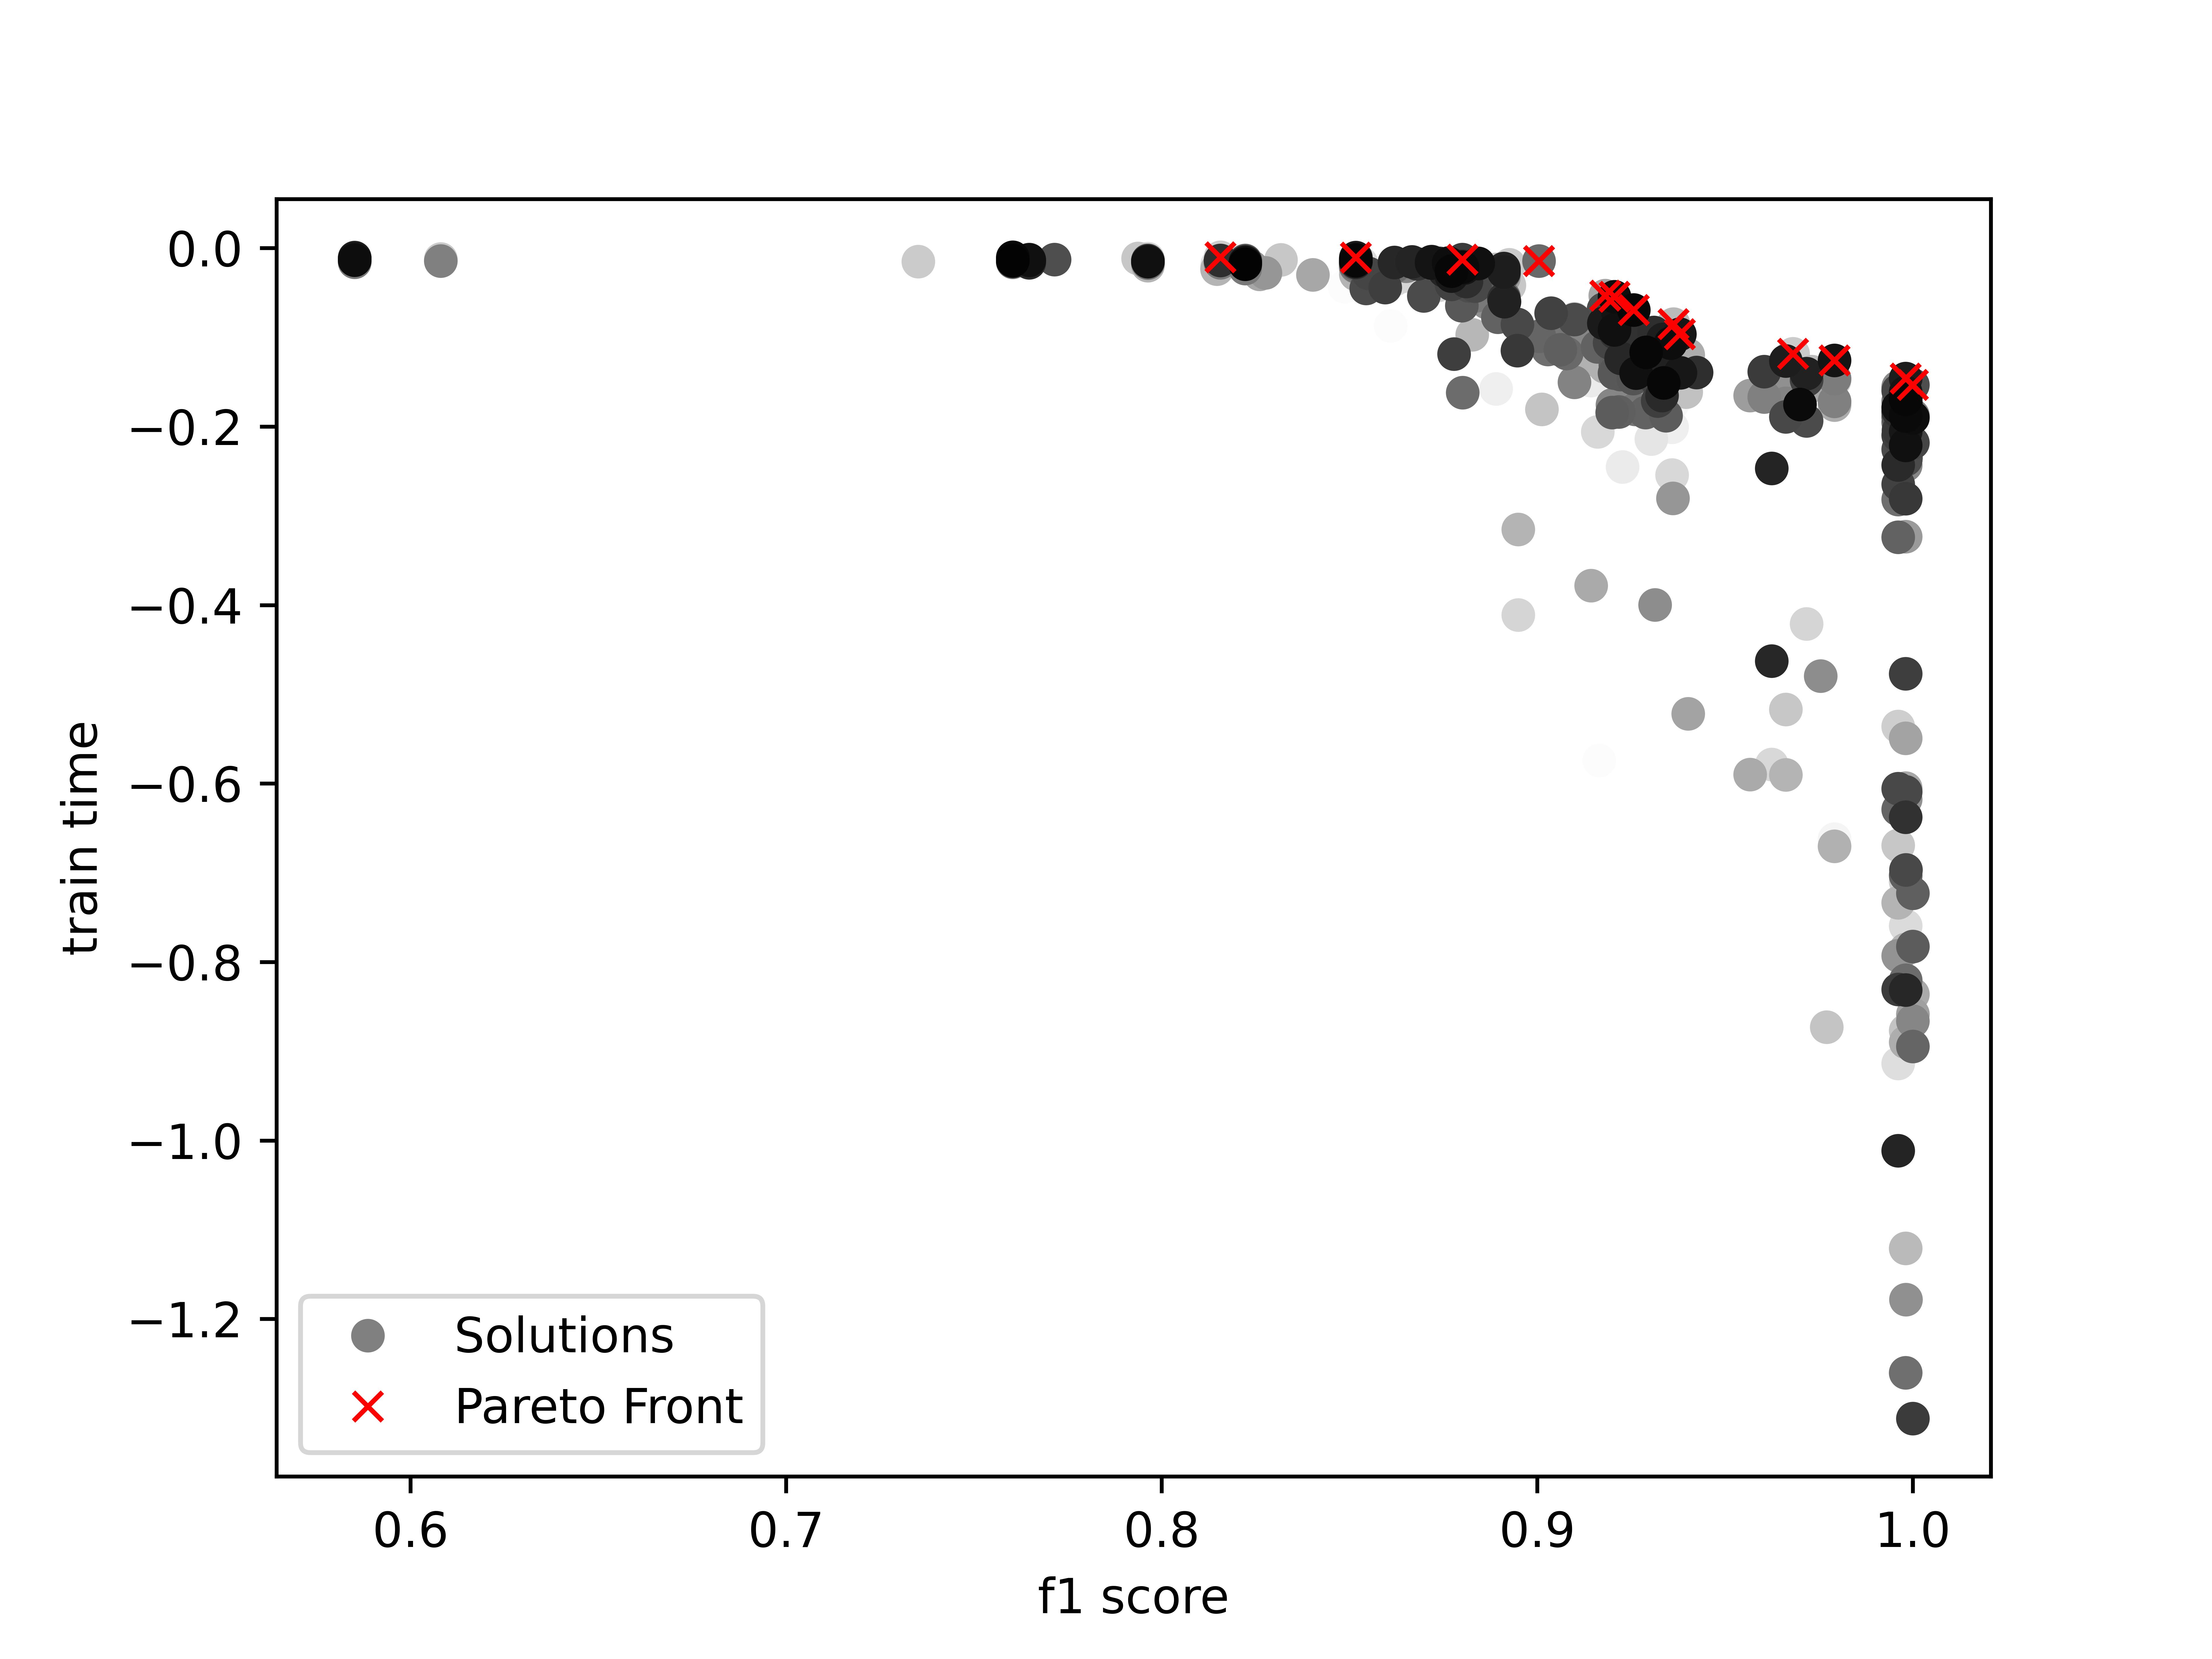
\includegraphics[scale=0.8]{Pictures/cars_fscore_vs_time.jpg}
    \caption{Cars: f-score contra tiempo de entrenamiento}
    \label{impl:fig:cars:fscore_vs_time}
\end{figure}


\subsubsection{Precisi\'on contra Recobrado}

Este es un caso donde las m\'etricas a evaluar no entran en conflicto y no hay que hacer trade offs entre estas. Como se observa en \ref{impl:fig:cars:precision_vs_recall} el frente de Pareto esta consituido por un s\'olo punto tal que precision y recobrado son ambos el maximo. Se observa como en el transcrso de las generaciones las soluciones se acercan cada vez m\'as al frente de Pareto.

En este caso especif\'ico AutoGOAL encontr\'o 30 soluciones distintas con respecto a algoritmos e hyperpar\'ametros que logran este rendimiento. Puede haber ocasiones donde esto sea interesante para el usuario desde un punto de vista investigativo, ver en que difieren.


\begin{figure}[ht]
    \centering
    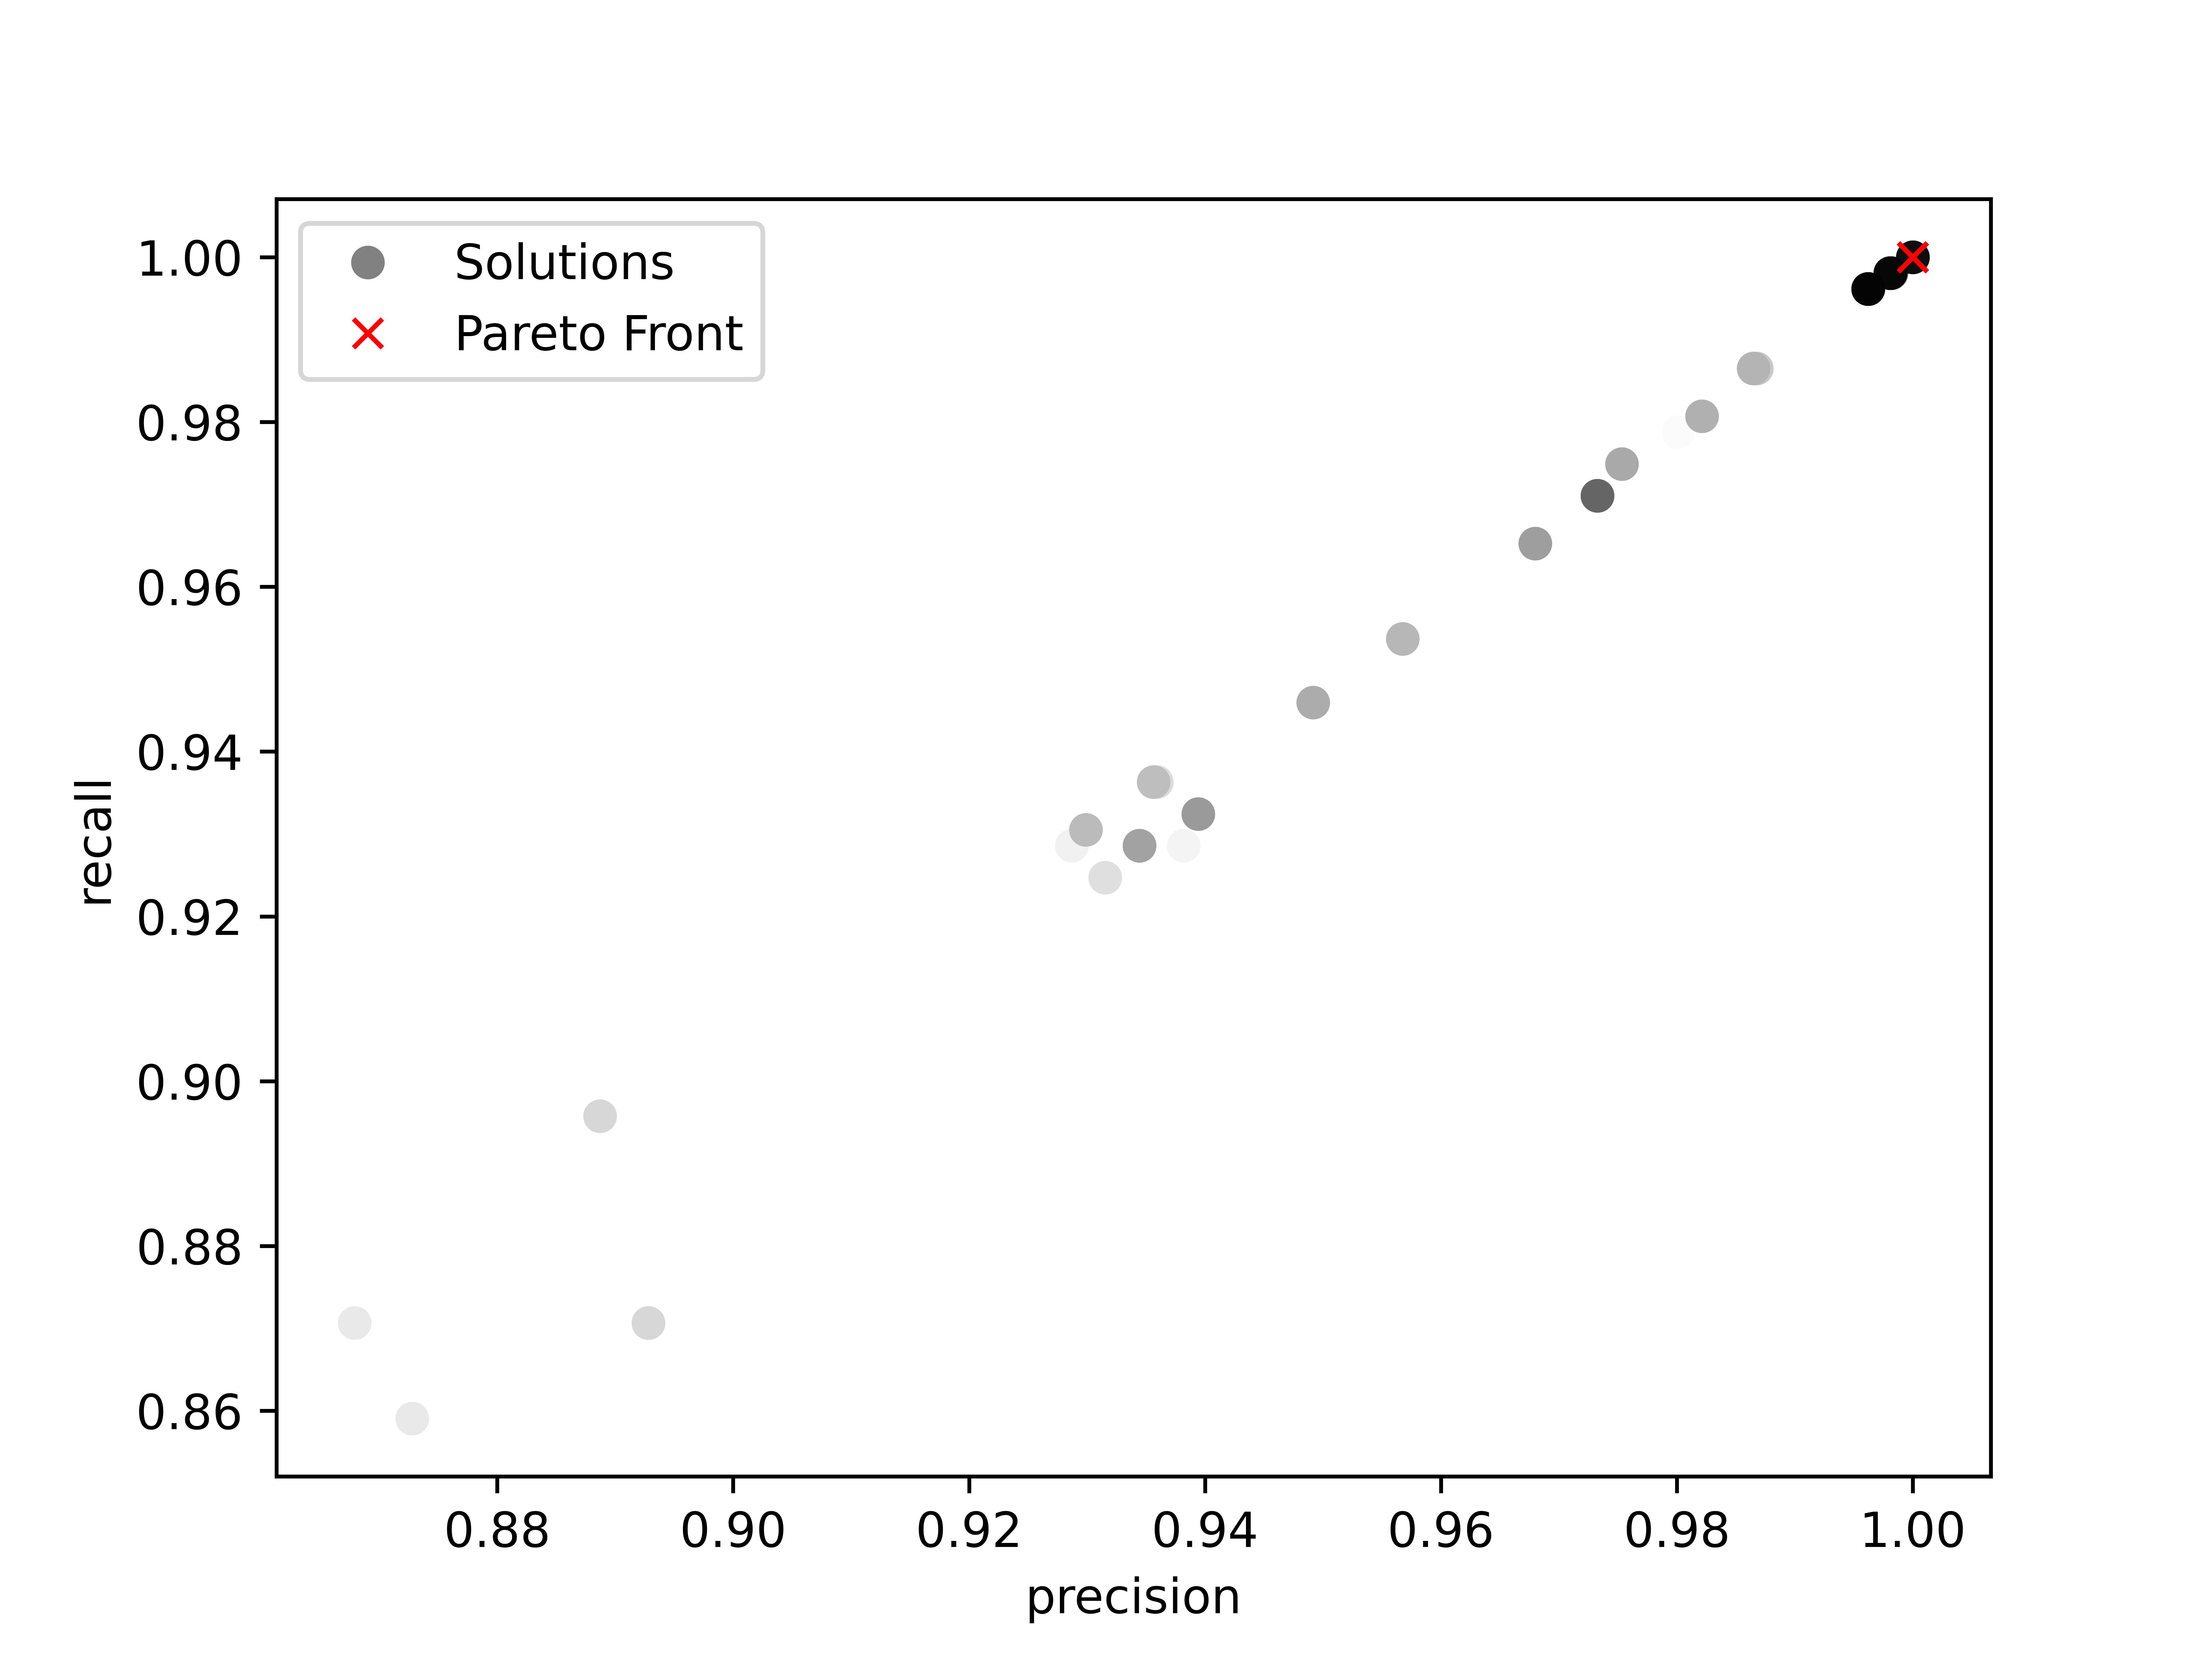
\includegraphics[scale=0.8]{Pictures/cars_precision_vs_recall.jpg}
    \caption{Cars: Precisi\'on contra recobrad}
    \label{impl:fig:cars:precision_vs_recall}
\end{figure}

\subsection{HAHA}

Se utilzo una poblacion total de 40 individuos, 8 horas de tiempo m\'aximo y 10 segundos por  evaluaci\'on. Las implementaciones de F-Score, Precision y Recall son las implementadas en Scikit con un promedio binario (el estandar) ya que es un problema de clasificaci\'on binario.

\subsubsection{F-Score contra Tiempo de Entrenamiento}

En \ref{impl:fig:haha:fscore_vs_time} se observa un frente con una aparente forma similar al de \ref{impl:fig:cars:fscore_vs_time}. Los pipelines de AutoGOAL en esta ocasi\'on est\'an conformados por dos algoritmos principales. Los que contienen poca precisi\'on pero son general m\'as rapidos est\'an conformados por HasingVectorizer y NearestCentroid y  lo que varia entre ellas son los hiperparametros. Los que tienen mayor precision a costo de un poco de tiempo est\'an compuestos por count vectorizer  y regresores log\'isticos.

Adem\'as en la esquina superior izquierda se ve como AutoGOAL busca un punto que tiene f-score 0, cosa que es completamnete innecesaria, pero el algorimto es agn\'ostico a esto. Ser\'ia recomendable añadir posibles restricciones a las b\'usquedas multiobjetivos para que el algoritmo no pierda poder de computo en buscar soluciones in\'utiles.

Por \'ultimo note que existen algorimtos usan el tiempo m\'aximo de 10 segundos ya que ese es el tiempo m\'aximo de evaluaci\'on dado. Ser\'ia intersante ver que sucede cuando se remueve esta limitaci\'on.

\begin{figure}[ht]
    \centering
    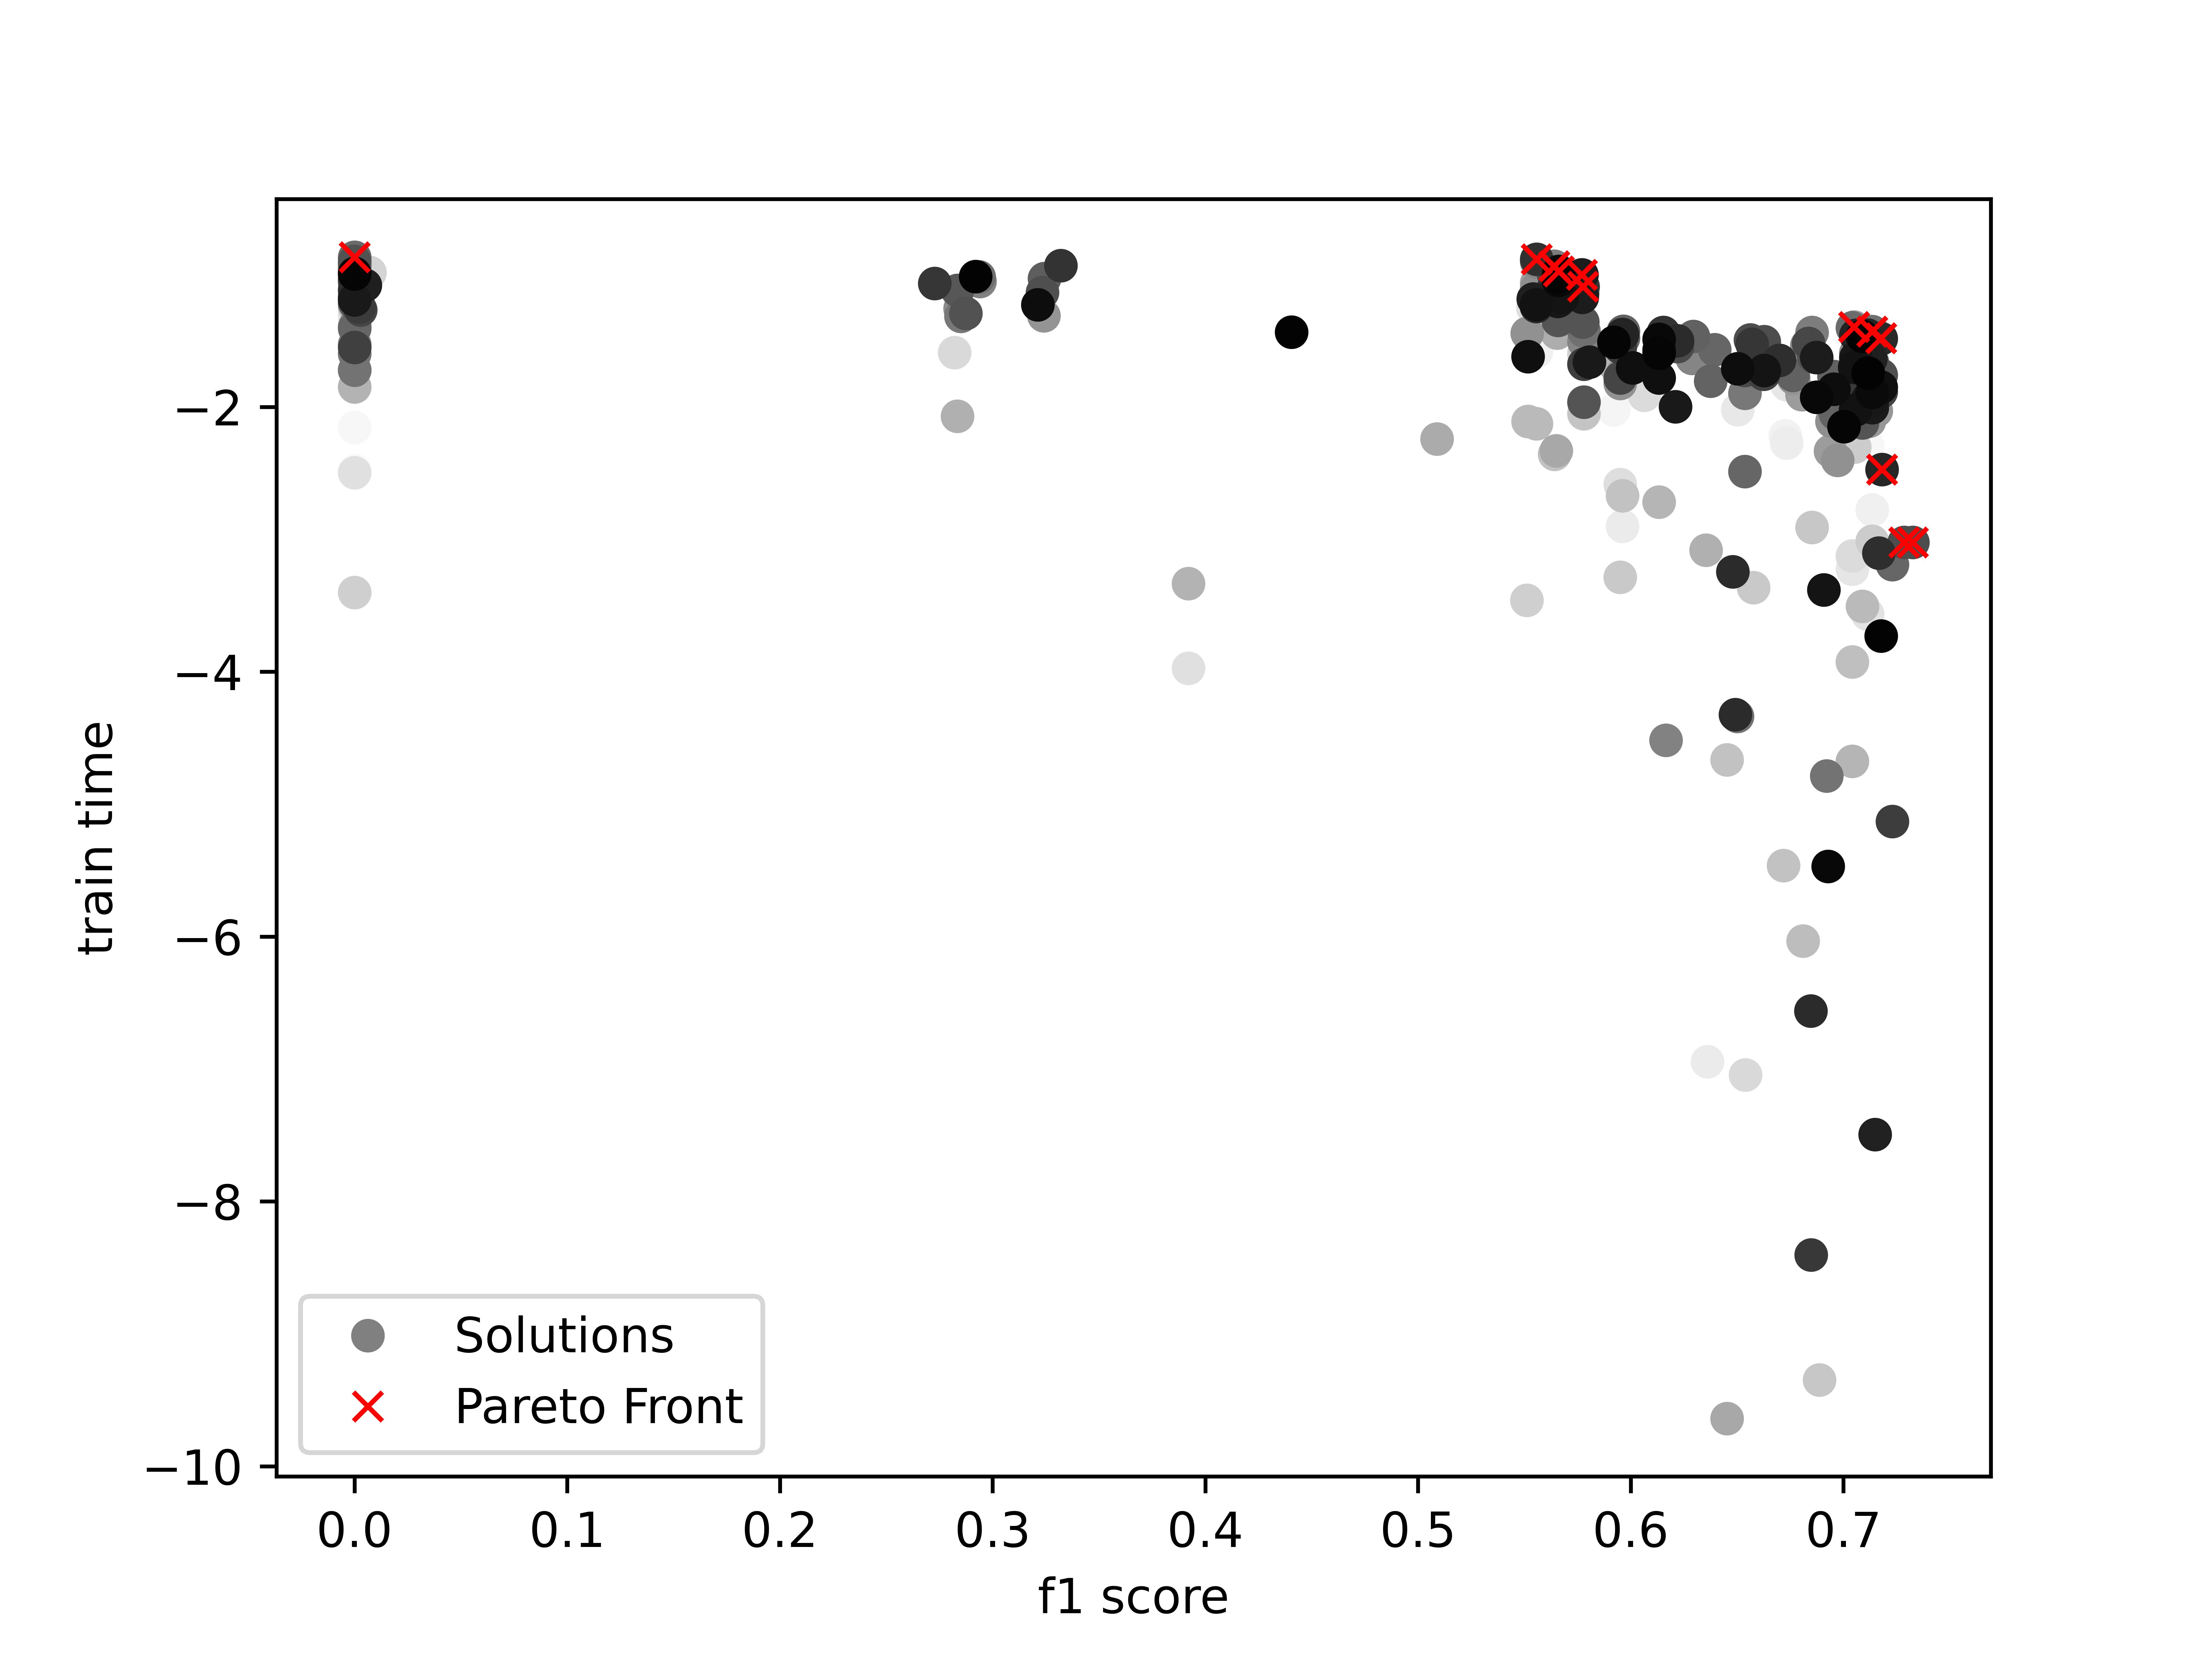
\includegraphics[scale=0.8]{Pictures/haha_fscore_vs_time.jpg}
    \caption{HAHA: F-score contra tiempo de entrenamiento}
    \label{impl:fig:haha:fscore_vs_time}
\end{figure}
\subsubsection{Precisi\'on contra Recobrado}

Contrario a lo que muestra la evaluaci\'on de Cars con respecto a precision y recobrado, no es posible encontrar un flujo que maximice a ambas y se empiezan buscar modelos que ofrezcan trade offs. Se pueden encontrar con buen recobrado y mala precision, dando y dando, o mal recobrado y muy buena precisi\'on. Este tambien tiene la forma de un frente convexo .

\begin{figure}[ht]
    \centering
    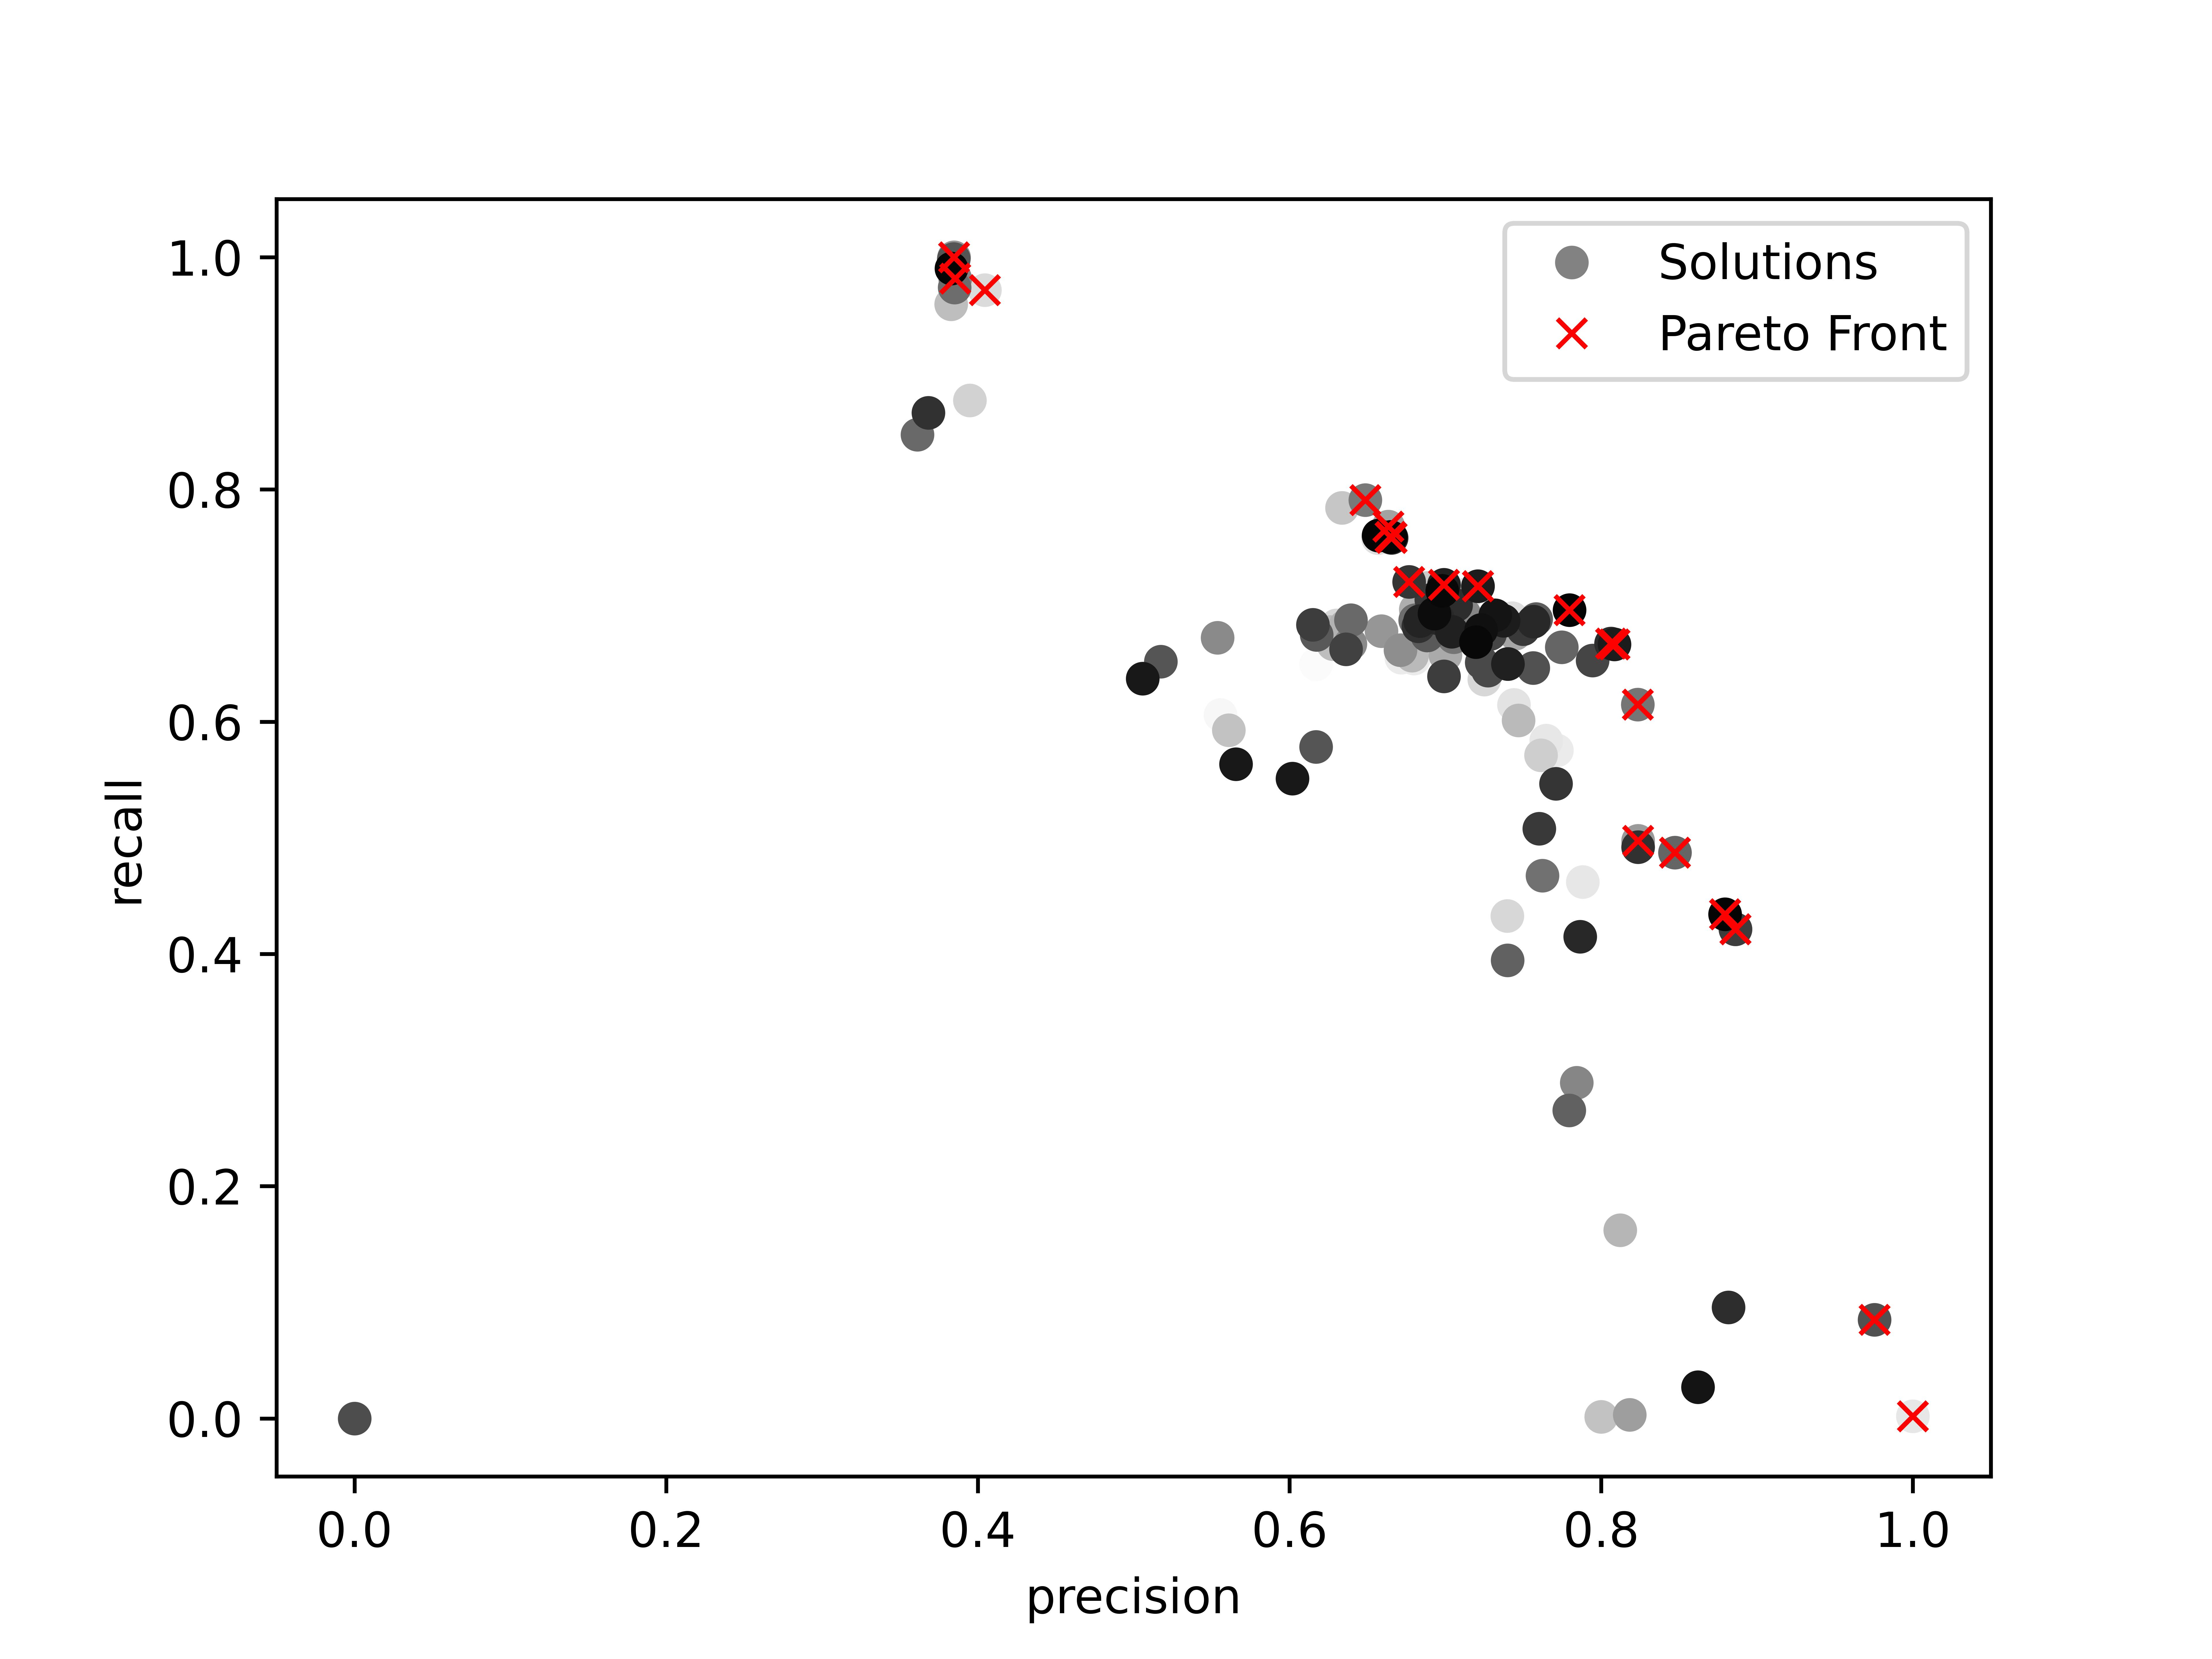
\includegraphics[scale=0.8]{Pictures/haha_precision_vs_recall.jpg}
    \caption{HAHA: Precisi\'on contra recobrado}
    \label{impl:fig:HAHA:precision_vs_recall}
\end{figure}

\subsection{MEDDOCAN}

Se utilzo una poblacion total de 5o individuos, 10 horas de tiempo m\'aximo y 10 mintuos por  evaluaci\'on. Las implementaciones de F-Score, Precision y Recall son las mismas versiones que vienen acompa\~nadas con el m\'odulo de Python que trae consigo el corpus de datos.

Aqu\'i el tiempo m\'aximo es mucho mayor pues es un corpues mucho m\'as grande que los anteriores que para encontrar al menos un pipeline v\'alido require alrededor de 7 u 8 minutos. Lo suficiente para lograr 3 o 4 generaciones de un total de 100.


\subsubsection{F-Score contra Tiempo de Entrenamiento}


\subsubsection{Precisi\'on contra Recobrado}

% Y despues de las pruebas

% Aqui lo que se me ocurre es poner casos de comparacion:
% Probar con tiempo de entrenamiento vs sin tiempo de entrenamiento
% Probar con precision y recall vs fscore
% Probar con otra m\'etrica como Interpretabilidad o Robustez

% Probar cuando se usan varias m\'etricas (para este s\'abado)

% Plotear como se acerca al frente de Pareto
